\chapter{Démarche adoptée et réalisations au sein de PPIL}
\label{chap:premierchapitre}

% --> A ajouter : 
% présentation de PPIL
% indicateurs intéressants. dans montée en compétence : Un projet de gestion de projet
% retour PMO
% mieux rédiger TNR
% mieux rédiger ANO
% vu toute la production d'un projet
%CNAM Métier
%HP ALM

\section{Montée en compétence sur le fonctionnel du projet}

Pendant ma première semaine de stage, j'ai effectué une montée en compétence sur le fonctionnel du projet. Il est important de souligner que j'ai continué à en apprendre toujours d'avantage sur le fonctionnel du projet tout le long de mon stage que ce soit en qualification ou en développement.

Dans cette section, je vais décrire ma démarche pour m'imprégner du projet. Il est évident que cette montée en compétence a été primordiale pour la suite de mon stage.

Pour cela, j'ai utilisé plusieurs méthodes :

Tout d'abord, j'ai étudié les spécifications fonctionnelles et technique du Projet, je me suis aussi procuré le manuel utilisateur de l'application auprès de l'équipe.

Au cours de cette montée en compétence, j'ai posé des questions aux différents analystes fonctionnels du projet, j'ai donc pu bénéficier de les explications des sachant sur le projet : le client, le contexte du projet ainsi que l'histoire de PPIL. 

Quelques informations importantes que j'ai pu recueillir lors de mon arrivée dans l'équipe :
\begin{itemize}
    \item Début de PPIL en 2010, 
    \item Refonte du projet en 2017, 
    \item Exigences du client,
    \item Des sprints qui durent 3 semaines, 
    \item Les besoins et les outils du client (les différents acteurs de la Cnam utilisent MSP),
    \item Comprendre les différentes fonctionnalités de PPIL,
    \item PPIL et les autres projets de la CNAM : on retrouve dans PPIL tous les autres projets de la Cnam,
    \item PPIL est intégré dans SharePoint car les agents de la CNAM manipulent des documents dans leur Sharepoint et le fait d'avoir PPIL dans une même structure leur permet de rassembler plusieurs outils au même endroit.
    \item Fonctionnement du Reporting de PPIL, 
    \item Différents concepts : indicateurs, jalons, diagrammes, lots, projet de référence, projets contributeurs.
\end{itemize}

En plus de ces explications et cette étude des documents, j'ai pu manipuler l'application PPIL, la prendre en main afin de me mettre à la place des utilisateurs finaux et de comprendre comment et pourquoi ils utilisent cet outil qu'est PPIL.

Il a été important de me mettre à la palce des différents profils d'utilisateurs de PPIL :
\begin{itemize}
    \item Chef de projet
    \item Manager
    \item Responsable DSI...
\end{itemize}

A la fin de la semaine, j'ai réalisé une présentation du projet et de ses fonctionnalités aux membres de mon équipe. La présentation a duré 10 minutes, cette présentation a eu pour objectif de présenter tout ce que j'ai appris sur le projet durant la semaine. A la suite de cette présentation, nous avons échangé avec les BA, RT et le chef de projet afin de préciser certains points important dans l'objectif d'en l'objectif que j'en sache un maximum sur le projet.

\subsection{Des indicateurs intéressants en terme de gestion de projet}

Dans cette partie je vais expliquer pourquoi PPIL est très intéressant en terme de gestion de projets. Il permet de voir comment une organisation (la Cnam) gère une multitude de projets.

J'ai découvert dans PPIL le mécanisme de reporting de projets et de lots ainsi que des indicateurs qui permettent de :
\begin{itemize}
    \item Planifier les projets dans le temps (notamment grace aux concept de jalon),
    \item Maîtriser et piloter les risques,
    \item Gérer un grand nombre de projets,
    \item Suivre des enjeux opérationnels de projets ou de lots,
    \item S'adapte en fonction des différents acteurs intervenant dans la gestion de projets.
\end{itemize}

\subsubsection{Visualiser les indicateurs en fonction du profil}

PPIL permet aux différents profils d'utilisateurs de visualiser les informations opérationnelles de leurs projets.

Pour les profils Chef de projet, Manager, Responsable DSI et MOA, on peut visualiser :
\begin{itemize}
    \item Visualiser l’indicateur \textbf{Bulletin de santé}
    Les projets dont la tendance est en dégradation et/ou la météo est orageuse sont mis en évidence par cet indicateur.
    \item Visualiser l’indicateur \textbf{Dérive des jalons}
    \begin{itemize}
        \item Les projets dont le prochain jalon et/ou la date de mise en production est en dérive sont mis en évidence par cet indicateur.
        \item Un jalon est en dérive lorsqu’il existe une différence de plus de 7 jours entre les dates du dernier reporting et de celui fait il y a un mois.
    \end{itemize}
    \item Visualiser l’indicateur \textbf{Avancement par phase} (Chef de projet)
    Les jalons de tous les projets aux états « En cours » du périmètre sont représentés dans cet indicateur.
    \item Visualiser l’indicateur Plan de charge équipe (Manager)
    En cliquant sur le graphique, on accède au rapport du Capacity Planning
    \item Visualiser l’indicateur \textbf{Planning des MEP} (mise en production) : Responsable DSI et MOA
    Les lots dont la date de mise en production est comprise entre le mois passé et les six prochains mois sont placés sur une échelle de temps.
\end{itemize}

\begin{figure}[h]
\centering
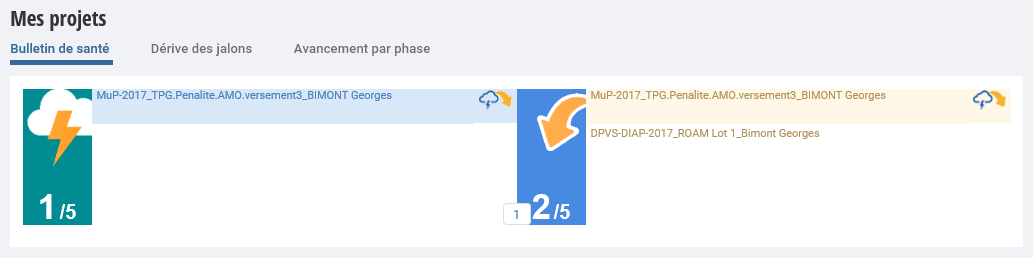
\includegraphics[width=1\textwidth]{images/ppil-bulletion-de-sante.PNG}
\caption{PPIL : Bulletin de santé (Profil Chef de Projet)}
\end{figure}

\subsubsection{Accéder aux reporting / restitution d'un lot / projet}
Pour rappelle, un lot contient plusieurs projets. Dans les indicateurs dans lesquels sont affichés les noms des projets, en cliquant sur le nom d’un projet :
\begin{itemize}
    \item En tant que Manager, Responsable DSI et MOA, on accède à la restitution du reporting
    \item En tant que CP, on accède à la saisie du reporting
\end{itemize}
En accédant au reporting d'un projet, on accède à différents indicateurs intéressants pour un lot/projet : 

\begin{figure}[!h]
\centering
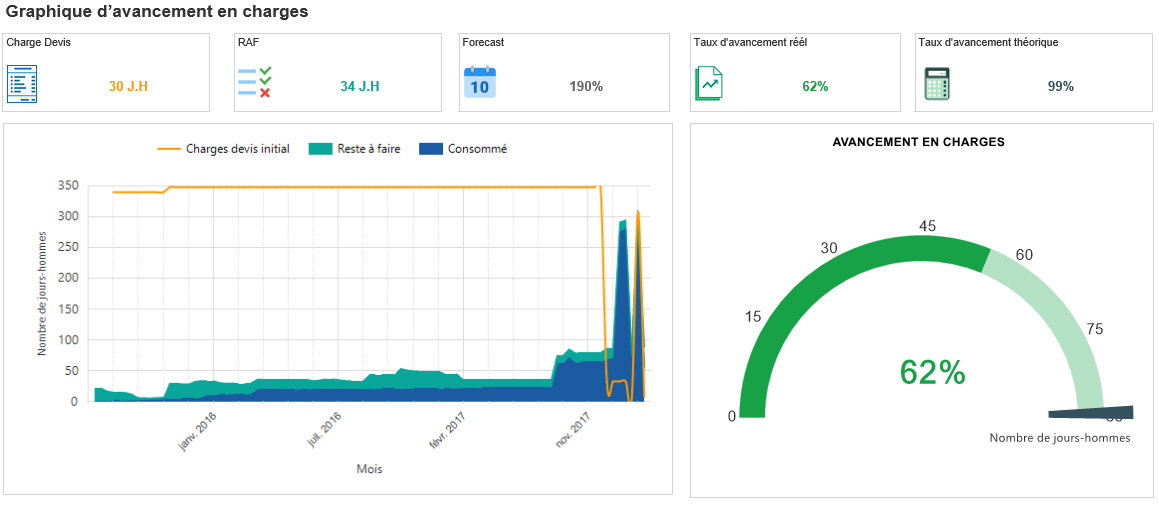
\includegraphics[width=1\textwidth]{images/PPIL-avancement.png}
\caption{PPIL : Graphique d'avancement en charges}
\end{figure}


\begin{figure}[!h]
\centering
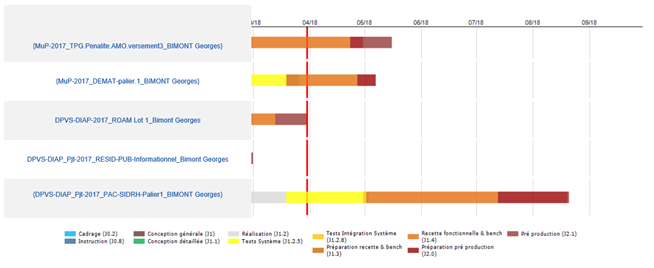
\includegraphics[width=2.5\textwidth]{images/PPIL-Gantt.png}
\caption{PPIL : Gantt des projets contributeurs}
\end{figure}

\begin{figure}[H]
\centering
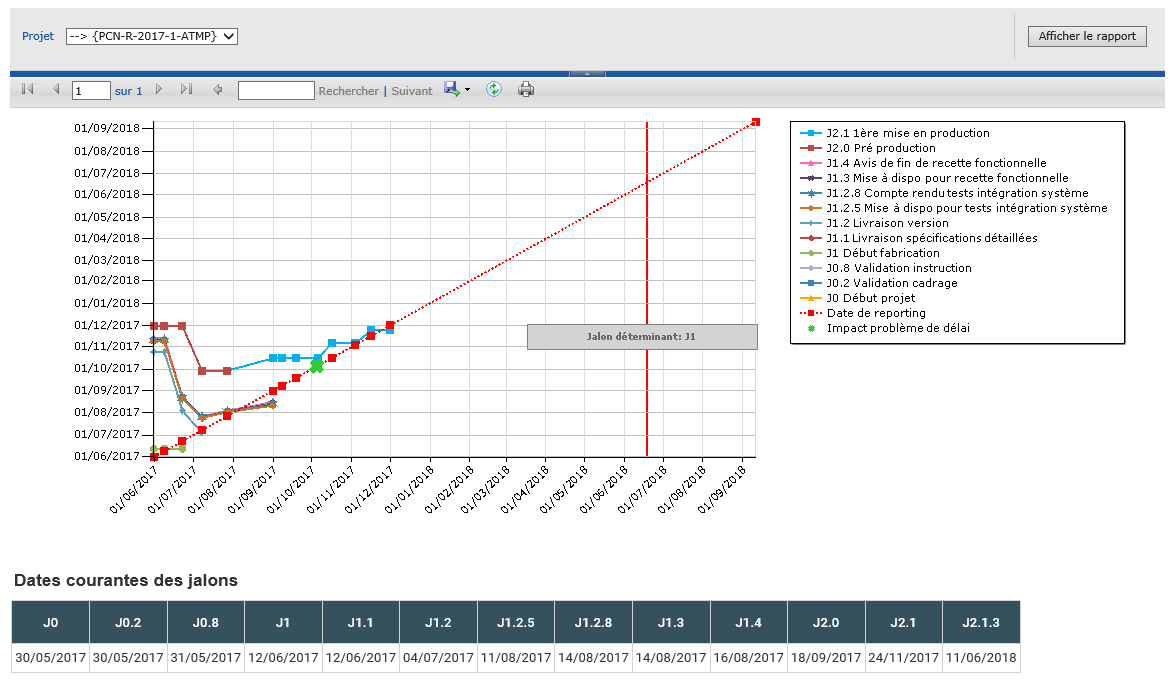
\includegraphics[width=0.8\textwidth]{images/temps temps.png}
\caption{PPIL : Capacity Planning}
\end{figure}

\subsubsection{Exécuter les actions rapides liées à mes projets}
Les actions rapides qui peuvent être effectués en tant que chef de projet sont \textbf{atteindre reporting} et \textbf{Actualiser les données MSP}, et en temps que Manager, on peut visualiser le nombre de notes de conjoncture à mettre à jour.

\subsubsection{Accéder à mes « informations opérationnelles » (CP, Manager, Responsable DSI et MOA)}
Gérer les actions de mes projets
Consulter les actions
Consulter les Facteurs de risque / problèmes
Consulter mes rapports opérationnels
Accéder aux « Rapports »


\section{La qualification}

Une partie de mon stage est destinée à la qualification, j'ai effectué différents tests :
\begin{itemize}
    \item Tests fonctionnels
    \item Tests de Non Régression
    \item Plan de tests
\end{itemize}

\subsection{L'importance des tests}

Durant mon stage, j'ai réalisé des tests afin de vérifier le bon fonctionnement des nouvelles fonctionnalités et corrections du projet ayant pour objectif de détecter d'éventuels anomalies ou régressions. Ces tests m'ont été bénéfique pour comprendre PPIL en profondeur. En effet, pour chaque tests, il faut comprendre et manipuler la base de données du projet, consulter les spécifications techniques ou fonctionnelles (SFG, STD) et poser des questions aux différents membres de l'équipe.

Au cours de ces tests, j'ai rencontré plusieurs difficultés : 

\begin{itemize}
    \item Certaines fonctionnalités à tester ne sont pas évidente à comprendre ou à reproduire.
    \item Les principes de l'outil : par exemple la logique de reporting en fonction des différents indicateurs.
    \item Manipuler une base de donnée complexe. (préparer des jeux de données, changer d'utilisateur, vérifier des informations en base)
\end{itemize}

A chaque fois, ces tests ont été effectués avant une livraison interne ou une livraison client.

Lors des tests il est important de prendre du recul et de tester d'autres fonctionnalités qui pourraient être impactées par la correction qu'on est en train de tester afin de détecter d'éventuels régressions.

Tous ces tests ont été réalisé grâce à l'outil HPALM.
        
Valider un test c'est prendre la responsabilité de dire qu'on peut livrer l'application. L'étape du test est primordiale, sans celle-ci un bon nombre d'erreurs ne seraient pas détectés.

\subsection{Les plans de tests}

J'ai eu l'occasion de rédiger des plans de tests. Cette étape demande une grande rigueur car il est important de couvrir tout le périmètre de la fonctionnalité à tester pour découvrir d'éventuels régressions. Ci-dessous un exemple de plan de test :

\begin{figure}[!h]
\centering
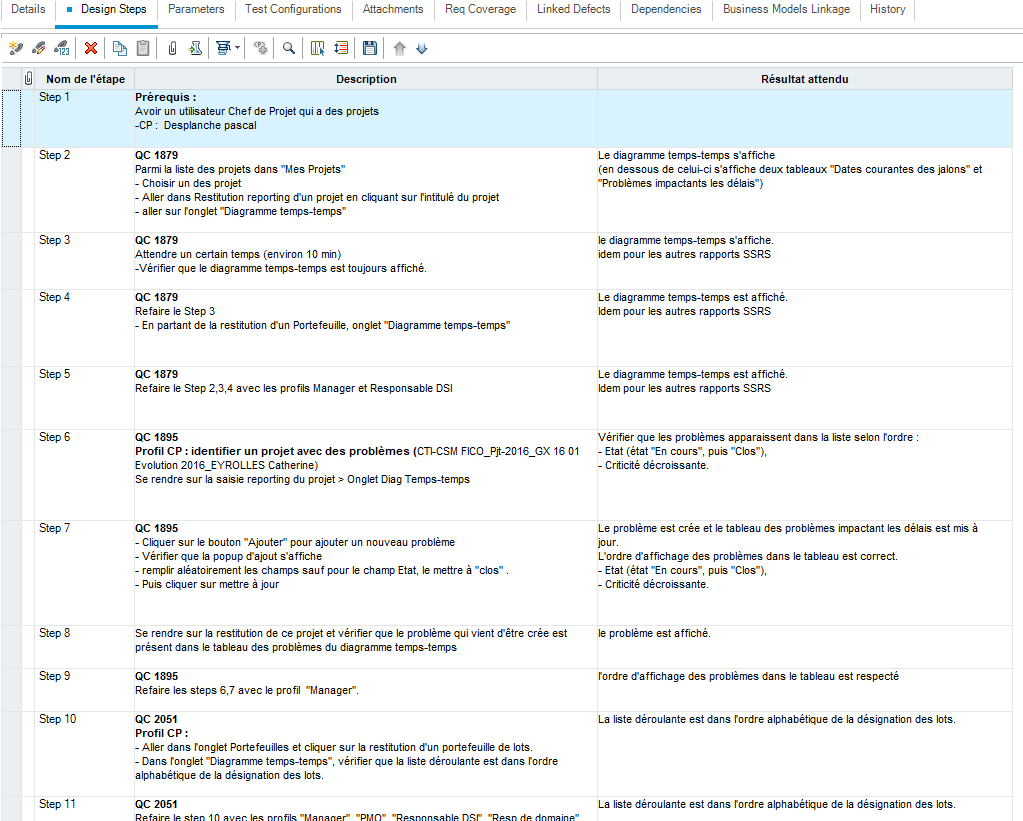
\includegraphics[width=0.8\textwidth]{images/HPLMplantest.png}
\caption{HP LM : Plan de test}
\end{figure}

\subsection{Un exemple de test réalisé : Les tests de Non Régression (TNR)}

[semaine 11/06]
Avant la livraison de la release 20.06.00. Il a fallut effectuer des tests de non régression.

Je vais décrire ici le test "06-TNR-ReportingRestitutionDuLot". Lors de ce test, j'ai détecté trois Defects. Ce qui a permis d'identifier et corriger une anomalie mineure, une anomalie majeure, et une régression majeure. Au cours de ce test de 40 steps, j'ai effectué un grand nombre de requêtes SQL, j'ai dû comprendre la logique de calcul ainsi que la logique d'affichage des indicateurs d'avancement d'un projet en fonction des jalons de celui-ci. Il a fallu que j'analyse la synchronisation des données projet entre Microsoft Project et PPIL.

\subsubsection{Difficultés rencontrées lors de ce test}
%capt ecran

description du step de ce test : 
vérifier que les indicateurs de suivi d'avancement des lots sont corrects :
Dans PPIL, dans la partie restitution de l'avancement d'un projet de référence. Dans cette partie il a fallu comprendre comment sont calculés les indicateurs de restitution pour l'avancement d'un lot. Pour cela j'ai consulté les SFD pour voir les règles de calcul. Je suis allé dans le code chercher les procédures stockées, après cela, j'ai fait mes calculs à l'aide de Excel et de SQL, n'ayant toujours pas le même résultat, j'ai demandé des explications à un BA notamment sur la synchronisation des données de MIcrosoft Project dans PPIL(outil utilisé par les CP de la Cnam pour mettre à jour les jalons de leurs projets). Et j'ai analysé une procédure stockée. Grâce à ces explications et à ces analyses j'ai réussi à ajuster ma requête. 


%Expliquer ce problème
De restitution qui importe les projets contributeurs (qui font parti du même PRT Palier).

Pour la partie Avancement en charge
\begin{figure}[h]
\centering
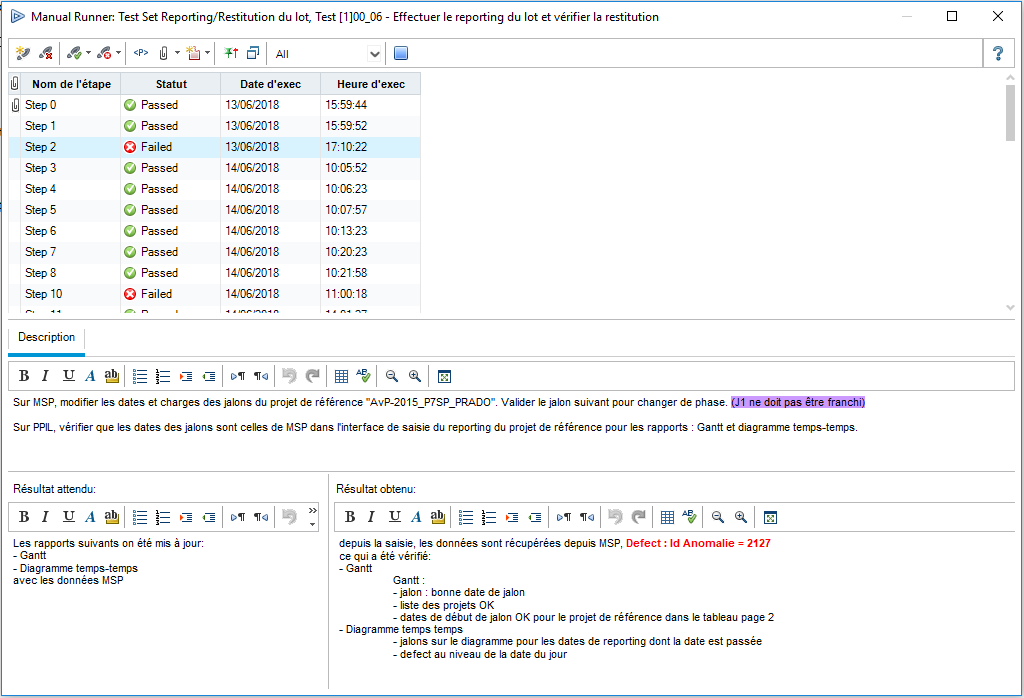
\includegraphics[width=0.8\textwidth]{HPALM-test.PNG}\\[1cm]
\caption{HP ALM : Déroulement d'un test}
\end{figure}

\section{Environnement technique du projet}

Pendant la deuxième semaine, j'ai également mis en place mon environnement de développement avec Achref (mon SB référent). Le projet PPIL se situe dans un contexte technique Microsoft. 

\begin{itemize}
    \item Sharepoint, 
    \item SQLServer, 
    \item .net
    \begin{itemize}
        \item C\#, 
        \item Telerik, 
        \item TypeScrypt, 
        \item Entity Framework, 
        \item SSRS, 
        \item HTML, 
        \item CSS etc).
    \end{itemize}
\end{itemize}

Outils utilisés :
\begin{itemize}
    \item Visual Studio
    \item HPLM
    \item Git
    \item Microsoft SQL Server Management
    \item Microsoft Team Foundation Server
\end{itemize}

\section{Développer au sein de PPIL}

J'ai commencé à développer au mois de Mai. Les développements au sein de PPIL se font en fonction de l'évolution du sprint en cours. Je suis arrivé dans un contexte de correction d'anomalie. C'est naturellement que des (QC) corrections d'anomalies m'ont été attribuées.

Ma première tâche a été de normaliser la charte graphique en même temps que l'interface du projet dans le but d'harmoniser les deux. Cette tâche fait suite à un retour du client (FT). Cela m'a permis de découvrir l'environnement technique. 

Ensuite, j'ai principalement corrigé des anomalies et développé quelques évolutions.

\subsection{Correction d'anomalies}

Lorsque les BA détectent une anomalie, ils l'identifient et la répertorie dans l'outil HPALM. Il est important de préciser que certaines anomalies sont détectées par le client. Elles sont classées par priorité et importance.
Les FT (anomalie retour client) sont souvent prioritaires par rapport aux anomalies détectés par l'équipe.
Un lot correspond à une version de l'application, chaque defect est rattaché à un lot.

\begin{figure}[h]
\centering
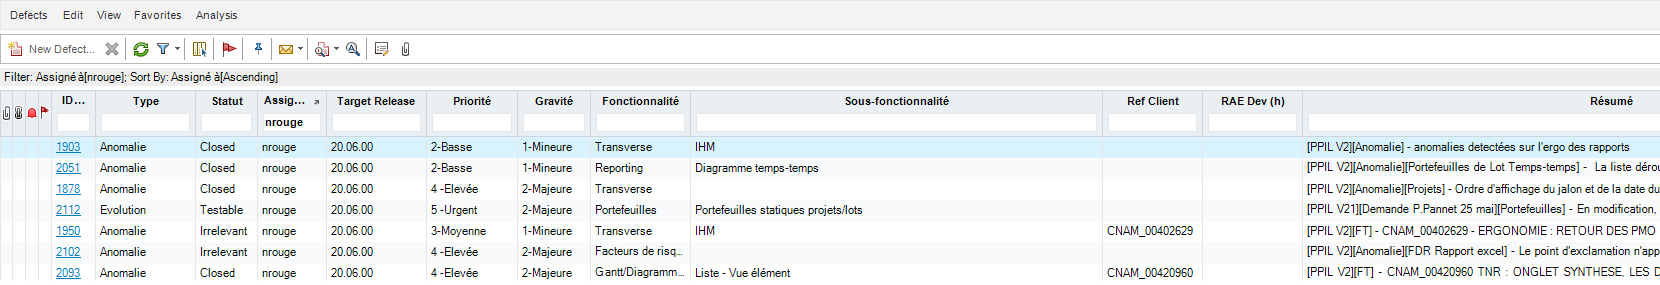
\includegraphics[width=1\textwidth]{images/HPLMliste.png}
\caption{HP LM : Defects corrigés de la release 20.06.00}
\end{figure}

\subsection{Démarche Adoptée}

Avant de commencer le développement, j'ai dû lire les consignes de code, règles à respecter soigneusement car mes développements seront livrés directement.

J'ai été chargé de corriger les anomalies distribuées par les RT.
Le référent technique a attribué différentes QC (Anomalies) aux différents SB. 
Les anomalies que j'ai corrigées étaienent toutes différentes et incluaient différentes technologies à chaque fois.

Quelques exemples d'anomalies que j'ai corrigés : 
\begin{itemize}
    \item Suppression d'un élément qui ne se supprime pas en base
    \item Erreur dans le chargement d'une page
    \item Bouton "annuler" non présent
    \item Ordre ou classement pas correct
    \item Direction de page incorrect lors de la consultation...
\end{itemize}

Pour mener à bien ces différentes corrections, il a été important de prendre du recul avant chaque correction. De bien identifier le périmètre du defect afin d'éviter les régressions.

Tout d'abord, j'ai du comprendre et analyser l'architecture du programme afin d'identifier plus facilement la provenance des defects. 

Chacun des points suivant ont été très important dans ma démarche de correction d'anomalie :
\begin{itemize}
    \item étudier l'architecture de la BDD a été primordiale pour avoir une visibilité sur les relations entre les différentes entités 
    \item me former sur les technos
    \item comprendre l'anomalie aussi bien fonctionnellement que techniquement
    \item analyser l'ampleur et périmètre de l'anomalie
    \begin{itemize}
        \item pour quel type d'utilisateur 
        \item dans quel mode (consultation, restitution, 
        \item dans quel rubrique ( mes projets, ptf, ...
    \end{itemize}
    \item identifier la provenance du problème

\end{itemize}

Comprendre la logique de développement :
\begin{itemize}
    \item comprendre pourquoi le projet a été codé de cette manière
    \begin{itemize}
        \item aller voir les développeurs, 
        \item aller voir le référent technique,
        \item consulter spécifications techniques ou fonctionnelles
    \end{itemize}
    \item identifier les solutions possibles
    \item choisir la meilleure façon de faire à :
    \begin{itemize}
        \item modifier au minimum le code,
        \item trouver la solution la plus optimale,
        \item éviter faire de régression 
    \end{itemize}
 \end{itemize}              
            
\subsubsection{Respect des délais (RAE)}
Pour chacune de mes tâches j'ai dû estimer le temps prévu à la réalisation de celle-ci. Respecter les délais est très important sur plusieurs points :
\begin{itemize}
    \item Pour le projet, cela sert de savoir quand on pourra proposer une version du projet au client.
    \item Pour l'équipe afin de savoir quelle tâche est assignée à quel développeur. 
    \item Pour moi, dans le choix de la démarche de résolution de la tâche.
\end{itemize}

Processus et outil utilisés :
\begin{itemize}
    \item Après avoir développé une évolution les étapes à suivre sont :
    \item "Pusher" ma branche avec git sur le dépot distant,
    \item Créer une "pull request" pour alerter le référent technique,
    \item Commenter la correction ou l'évolution sur HPLM
\end{itemize}

\begin{figure}[!h]
\centering
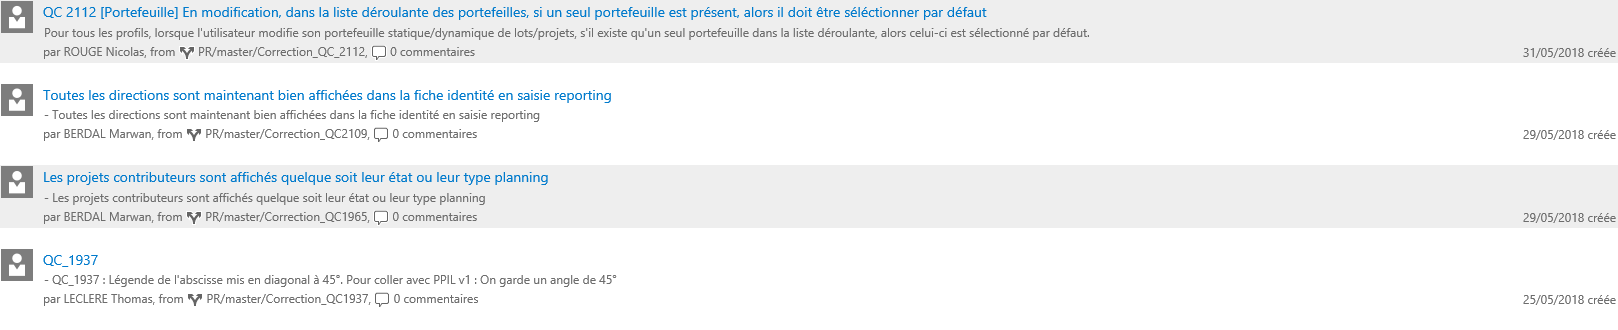
\includegraphics[width=1\textwidth]{images/PullRequest.png}
\caption{Visual Studio Team Foundation : Les Pull Request}
\end{figure}

Ci-dssous le workflow des anomalies dans HP ALM :
\begin{figure}[!h]
\centering
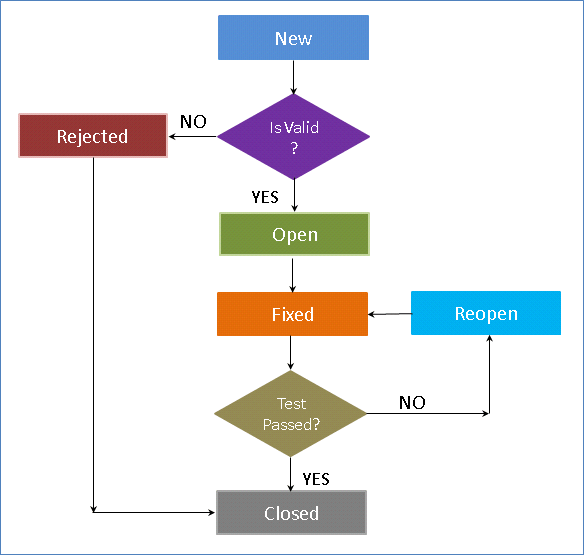
\includegraphics[width=0.6\textwidth]{images/DefectHPALM.png}
\caption{HP ALM Defect Workflow}
\end{figure}

\subsection{Quelques exemples d'anomalies corrigées}

Toutes les anomalies ont été intéressantes à corriger, et elles m'ont fait progresser et travailler sur des technologies diverses. J'ai réussi à acquérir les compétences techniques et nécessaires au projet. L'enjeu de la correction de ces anomalies c'est de n'avoir aucun retour bloquant en qualification interne et externe ainsi que de garantir la non régression.

\subsubsection{Anomalie [Poretefeuille][liste déroulante]}

Visuel de l'anomalie dans HPALM :
\begin{figure}[!h]
\centering
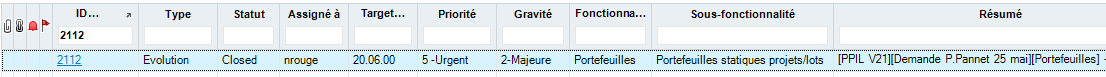
\includegraphics[width=1\textwidth]{images/QC2120.PNG}
\caption{HPALM : Defect 2112}
\end{figure}

On peut voir que l'anomalie est de priorité urgente et de gravité majeure, et qu'elle a été détectée par le client (priorité supplémentaire).

\textbf{Description de la correction à effectuer :} 

[Profil CP ou Manager][portefeuille]
Dans la liste déroulante qui apparaît lorsqu'on veut ajouter des projets ou des lots dans les différents portefeuilles de : 

\begin{itemize}
    \item lots statiques,
    \item lots dynamiques,
    \item projets statiques,
    \item projets dynamiques.
\end{itemize}

Sélectionner par défaut un portefeuille s'il n'y en a qu'un seul. Ne rien sélectionner par défaut sinon. 
[Profil Responsable DSI][portefeuille], Sélectionner par défaut "Mes projet favori" quelque soit le nombre de portefeuille existant.

Avant de commencer la correction du code de cette QC, j'ai mis au courant le référent technique que la description du defect était sujette à interprétation.Le RT a remonté l'information au client, qui a fait un retour en précisant le defect.

Lors de la correction en elle-même, j'ai du identifier ou faire les modification de code. Puis au cours de celle-ci j'ai pu monter en compétence sur du C\#, du Type-script ainsi que Kendo. J'ai du prendre en compte les différentes conditions pour réaliser différentes actions. 

\begin{figure}[!h]
\centering
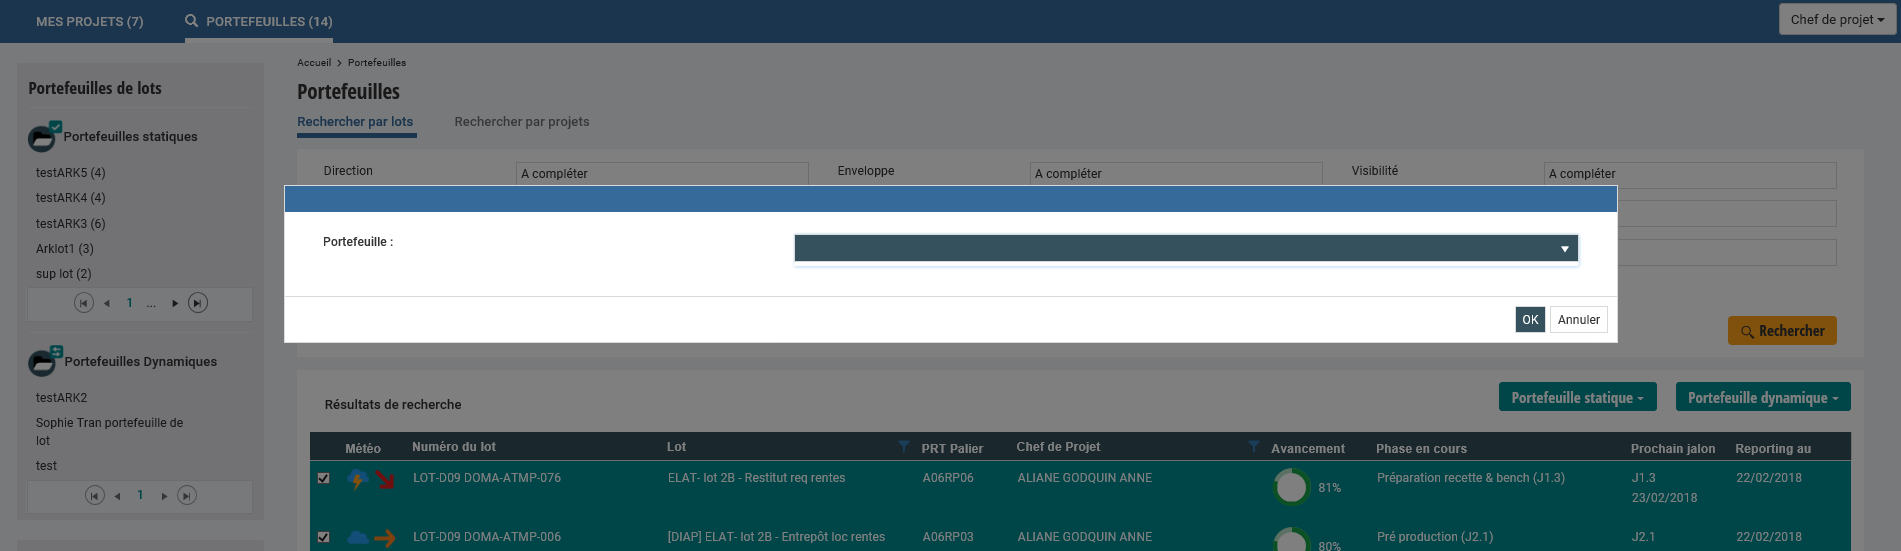
\includegraphics[width=1\textwidth]{images/correction1.PNG}
\caption{HPALM : Defect 2112}
\end{figure}

\subsubsection{Anomalie [Supression des lots non effective dans plusieurs cas]}

\textbf{Description de la correction à effectuer :} 
La suppressions des lots non effective selon certains critères :
\begin{itemize}
    \item Un lot ne se supprime pas quand il est dans un portefeuille (le lot se supprime visuellement mais pas en base, quand on refresh la page il réapparaît)
    \item Un lot ne se supprime pas quand il a des demandes rattaché
    \item Un lot ne se supprime pas quand il n'a pas de projet de référence
\end{itemize}

Cette anomalie m'a pris plusieurs jours de correction, les points importants à souligner sont : 
\begin{itemize}
    \item Il a fallut mettre en place plusieurs jeux de données pour visualiser l'anomalie.
    \item Pendant la correction j'ai détecté une autre anomalie : un lot sans projet de référence ne s'affiche pas dans un portefeuille. (Anomalie que j'ai corrigé par la suite.)
    \item J'ai proposé une solution efficace et correcte.
    \item Je suis allé voir Nicolas (le RT du projet), afin d'avoir son retour sur ma correction.
    \item Il m'a apporté son recul et son expérience en me proposant de refaire une partie de cette correction en modifiant une procédure stockée en SQL plutôt que de modifier une partie du code. Cette solution étant préférable pour la maintenabilité du code et de l'optimisation**.
\end{itemize}

Pour rappel, ce sont les PMO qui ont les droits pour supprimer des lots, un lot est constitué d'un ensemble de projets. Ci-dessous l'interface des PMO.

\begin{figure}[!h]
\centering
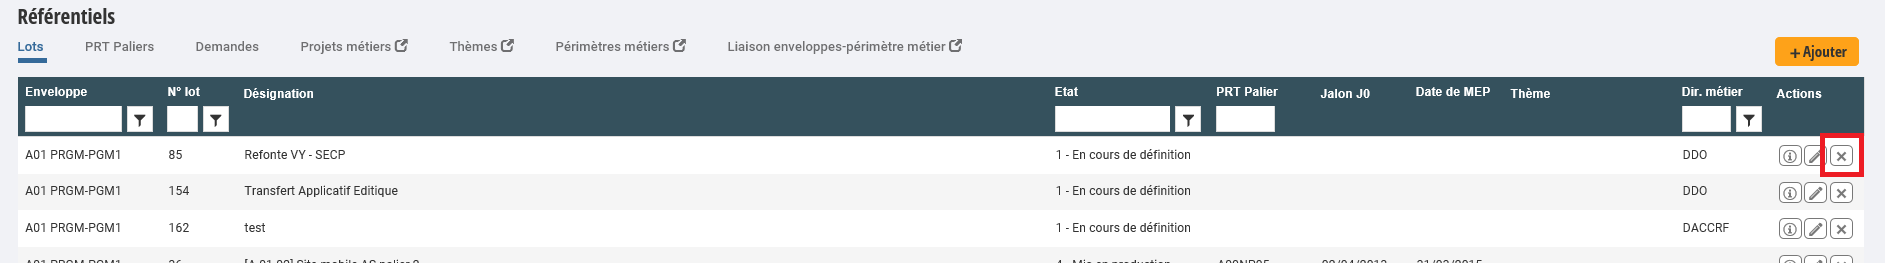
\includegraphics[width=1\textwidth]{images/ano2.png}
\caption{HPALM : Defect 2112}
\end{figure}


\subsubsection{Troisième anomalie }

\textbf{Description de l'anomalie :} En restitution d'un projet, onglet synthèse, quand on remonte sur une semaine précédente, les dates ne sont pas les bonnes. 

\begin{figure}[!h]
\centering
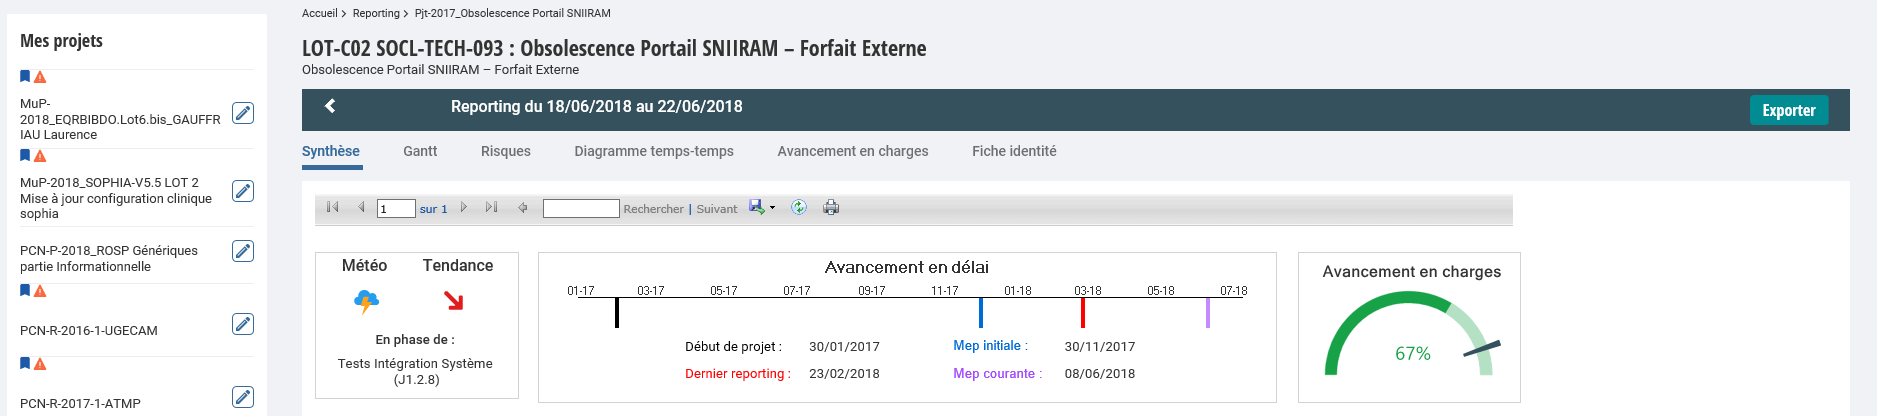
\includegraphics[width=1\textwidth]{images/ppil-indicateur-synthese.PNG}
\caption{Indicateur Synthèse}
\end{figure}

Les difficultés rencontrées lors de cette correction ont été :
\begin{itemize}
    \item Comprendre le fonctionnel, c'est à dire la logique des jalons.
    \item Travailler et modifier des requêtes complexes.
    \item Ne pas faire de régression.
\end{itemize}


\subsubsection{Des anomalies très complexes ** photo ?}

des requêtes très complexes qui vont chercher des données sur le CUBE, aucun membre de l'équipe ne maîtrise la techno, je suis chargé pendant une semaine d'analyser les ano et de trouver une correction. Un des développeur m'a rejoint pour chercher des solutions avec moi.


%%% Local Variables: 
%%% mode: latex
%%% TeX-master: "isae-report-template"
%%% End: 